\chapter{CERN, LHC e o Experimento ATLAS}

A Ciência procura compreender as leis que regem a Natureza. Uma das questões
mais antigas desta busca refere-se à constituição da matéria. A Física de
Partículas é a parte da física que estuda os constituintes da matéria e as
interações entre eles.

A matéria como conhecemos é formada por partículas estáveis. Há, porém,
partículas instáveis que duram apenas frações de segundos. Ambos tipos
coexistiram nos instantes posteriores ao \emph{Big Bang}.

É possível observar essas partículas instáveis utilizando os aceleradores de
partículas. Nesses aparelhos, um feixe de partículas, como prótons ou elétrons,
são aceleradas até altas velocidades, aumentando a energia cinética.  Quando a
energia chega ao patamar desejado, o feixe é colidido com outro grupo de
partículas, recriando assim as condições ideais para a formação de partículas
instáveis.

O CERN~(\emph{Organisation européenne pour la recherche nucléaire}) é o maior
laboratório de física de partículas do mundo e nele se encontra o mais complexo
aparato científico já construído pelo homem, o LHC~(\emph{Large Hadron
Collider})~\cite{EVANS2008}. Neste capítulo será apresentado este acelerador,
com enfoque no detector ATLAS e seus subsistemas.

\section{Breve Introdução ao Modelo Padrão}

O modelo atômico de Rutherford-Bohr, apresentado em 1913, é amplamente
conhecido. Nele prótons, nêutrons e elétrons são os componentes básicos dos
átomos. Esta noção é correta, porém existem partículas ainda menores. Hoje
sabe-se que tudo é formado pela combinação de 16 elementos fundamentais
classificados como \emph{quarks}, \emph{léptons} (\emph{férmions}) e os
mediadores de interações (\emph{bósons}).  O Modelo Padrão, publicado no final
da década de 1960, explica a função destas partículas bem como as que forças
atuam sobre elas~\cite{GRIFFITHS2008}. A Figura~\ref{fig:modelopadrao}
apresenta os elementos básicos desse modelo:

\begin{figure}[htpb!]
    \centering
    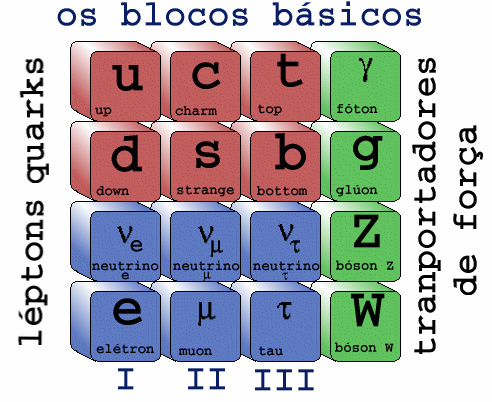
\includegraphics[width=8cm]{images/modelo_padrao.png}
    \caption{Modelo padrão de partículas elementares.}
    \label{fig:modelopadrao}
\end{figure}

Os prótons e nêutrons presentes no núcleo atômico  são compostos por
\emph{quarks}. Existem seis tipos de quarks frequentemente agrupados em duplas:
\emph{up}/\emph{down}, \emph{charm}/\emph{strange}, \emph{top}/\emph{bottom},
todos com seu \emph{anti-quarks} correspondentes. \emph{Quarks} nunca são
observados separadamente.Quando \emph{quarks} se agrupam, formam uma partícula
composta chamada hádron.  Hádrons podem ser separados em duas categorias:
bárions, formados por até três \emph{quarks}, e mésons, formados por um
\emph{quark} e um \emph{anti-quark}.  Prótons e nêutrons são tipos de bárions.

O Modelo também contém seis tipos de léptons: elétrons, múons, tau e seus
respectivos neutrinos. Assim como os \emph{quarks} possuem \emph{anti-quarks},
léptons possuem anti-léptons. Contudo, os léptons podem ser observados
isolados. Elétrons, múons e tau são partículas carregadas e possuem massa,
enquanto neutrinos não possuem carga e possuem pouquíssima massa.  O lépton tau
e o múon são extremamente pesados e altamente instáveis. Por isso, decaem
rapidamente em léptons mais leves.

Partículas mediadoras carregam uma discreta quantidade de energia de um
elemento para a outro. São elas os fótons, glúons e os bósons W e Z. Fótons
atuam em partículas carregadas, \emph{quarks} e léptons, exercendo a força
eletromagnética. Glúons atuam nos \emph{quarks} mantendo-os unidos. Já os
bósons $W^\pm$ e $Z^0$ representam a força fraca que atua tanto em léptons como em
\emph{quarks}.  A única força não incluída pelo Modelo Padrão é a
gravitacional. Existe a possibilidade que haja uma partícula graviton, ainda
não observada~\cite{PERKINS2000}.

\section{Organização Europeia para Pesquisa Nuclear}

O CERN localiza-se na fronteira entre a Suíça e a França, próximo a cidade de
Genebra. Foi fundado com o objetivo de criar um laboratório europeu para
pesquisa de física nuclear, em que seus países membros pudessem dividir as
despesas de seus aparatos e instalações. Estimulados pelas diversas organizações
internacionais nascentes na Europa pós-guerra, um grupo de cientistas formaram
um conselho provisório em 1952, base para a fundação da atual organização,
ocorrida dois anos depois~\cite{ACZEL2012}. A Figura~\ref{fig:scienceglobe} mostra o
Globo de Ciências e Inovação, construído na ocasião do quinquagésimo aniversário
de fundação do CERN.

Atualmente, o CERN é dirigido por 20 Estados membros europeus (a
Figura~\ref{fig:cernflags} representa as respectivas bandeiras localizadas sua
entrada principal do instituto).  Contudo, outros países não-membros colaboram
das mais diversas maneiras, inclusive o Brasil.  No total, existem cerca de
8.000 cientistas provenientes de 608 universidades, representando 113
nacionalidades~\cite{ref:cern_www}.

\begin{figure}[htpb!]
        \centering
        \begin{subfigure}[b]{0.45\textwidth}
                \centering
                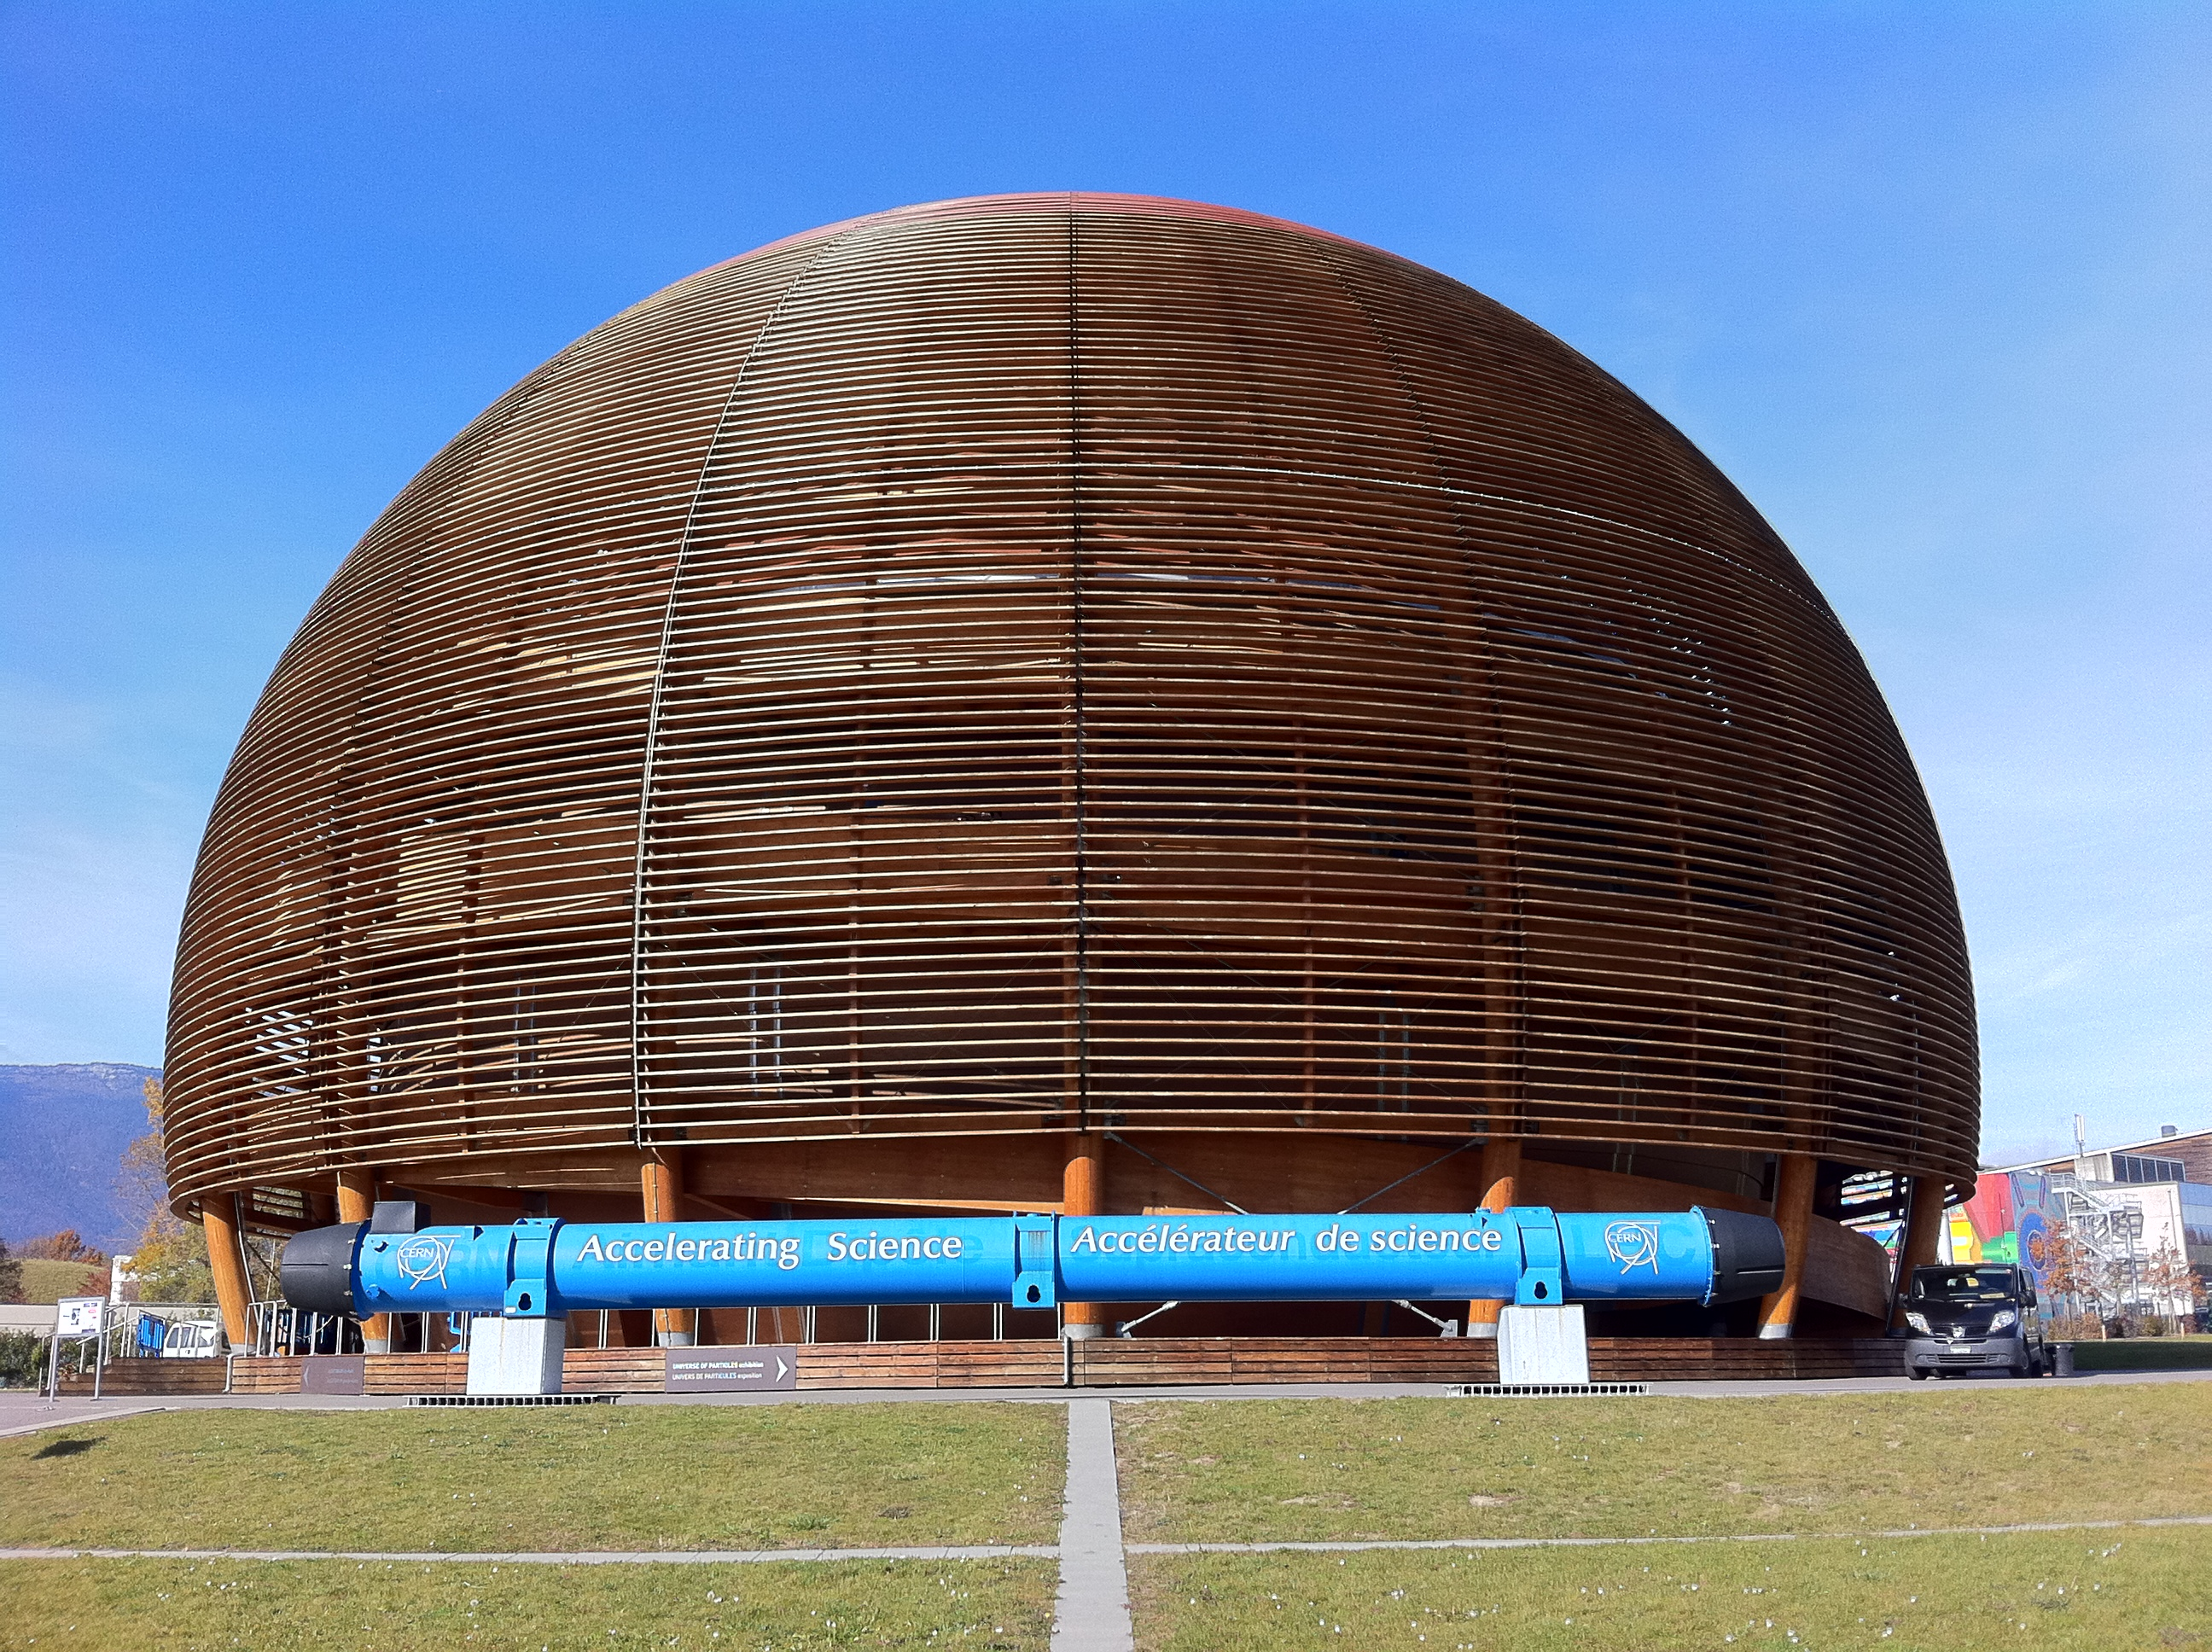
\includegraphics[trim=0cm 4cm 0cm 3cm, clip=true,width=\textwidth]{images/innovation_globe.jpg}
                \caption{ O Globo da Ciência e Inovação do CERN.}
                \label{fig:scienceglobe}
        \end{subfigure}%
        ~
        \begin{subfigure}[b]{0.45\textwidth}
                \centering
                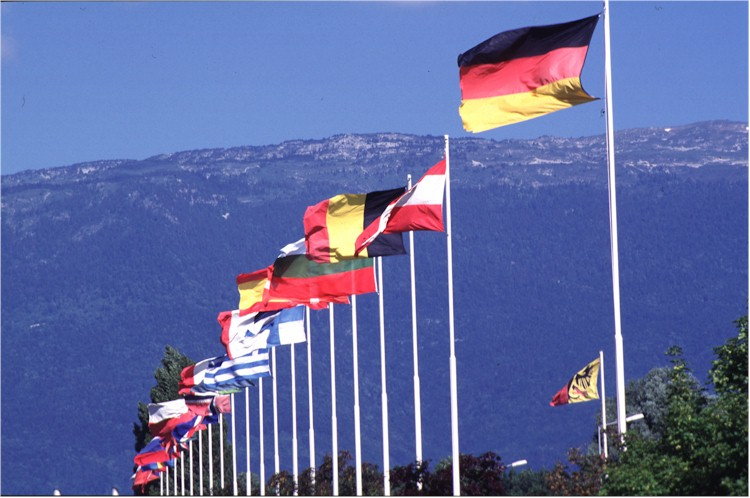
\includegraphics[width=\textwidth]{images/cern_flags.jpg}
                \caption{ Bandeiras dos países membros da organização.}
                \label{fig:cernflags}
        \end{subfigure}
        \caption[Fotografias de marcos no CERN.]{CERN: O maior laboratório de
        pesquisa nuclear do
        mundo (Imagens extraídas de~\cite{ref:cern_www}).}\label{fig:cern1}
\end{figure}

Além da colaboração à comunidade de física de partículas, o CERN contribui com
o desenvolvimento de tecnologias empregadas em diversas áreas. A invenção
da~\emph{World Wide Web}, equipamentos de imagens medicinais e a computação em
GRID são apenas alguns dos exemplos.

\section{O Projeto LHC (\emph{Large Hadron Collider})}

O LHC, o maior e mais poderoso acelerador de partículas do mundo, é o mais novo
aparato do complexo de aceleradores do CERN (Figura~\ref{fig:cerncomplex}). Ele
foi construído no túnel onde o LEP~\cite{ref:PICASSO1990} operou entre 1989 e
2000.  Esse túnel possui uma circunferência de 27~km de extensão e está
posicionado 150 metros abaixo da superfície. A Figura~\ref{fig:lhc} apresenta
um esquemático do anel do LHC e os principais experimentos localizados nele.

\begin{figure}[htpb!]
    \centering
    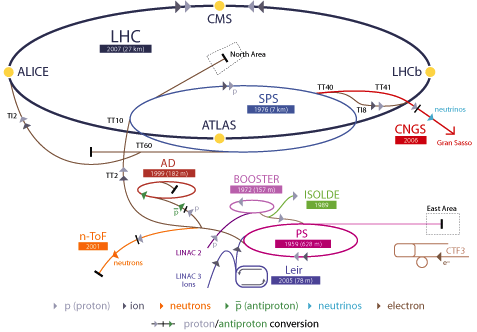
\includegraphics[width=12cm]{images/complexo_acelerador_CERN.png}
    \caption[Complexo de aceleradores no CERN.]{Complexo de aceleradores no CERN
    (Extraído de~\cite{ref:solans}).}
    \label{fig:cerncomplex}
\end{figure}

Antes de serem injetados com uma energia de 450~GeV no anel do LHC, prótons são
acelerados formando feixes. Esses feixes são acelerados até a energia
aumentar 15 vezes, adquirindo 7000~GeV~\cite{ref:solans}. Quando essa energia é
atingida, os feixes são colididos nos centro dos experimentos presentes ao longo
da trajetória.

O objetivo do projeto demanda uma elevada taxa de tomada de dados. O LHC opera a
40~MHz, ou seja, há a injeção de feixes a cada 25~ns. Operando na luminosidade
máxima projetada para o colisor, a taxa de eventos poderá alcançar
1~GHz~\cite{EVANS2008}.

\begin{figure}[htpb!]
    \centering
    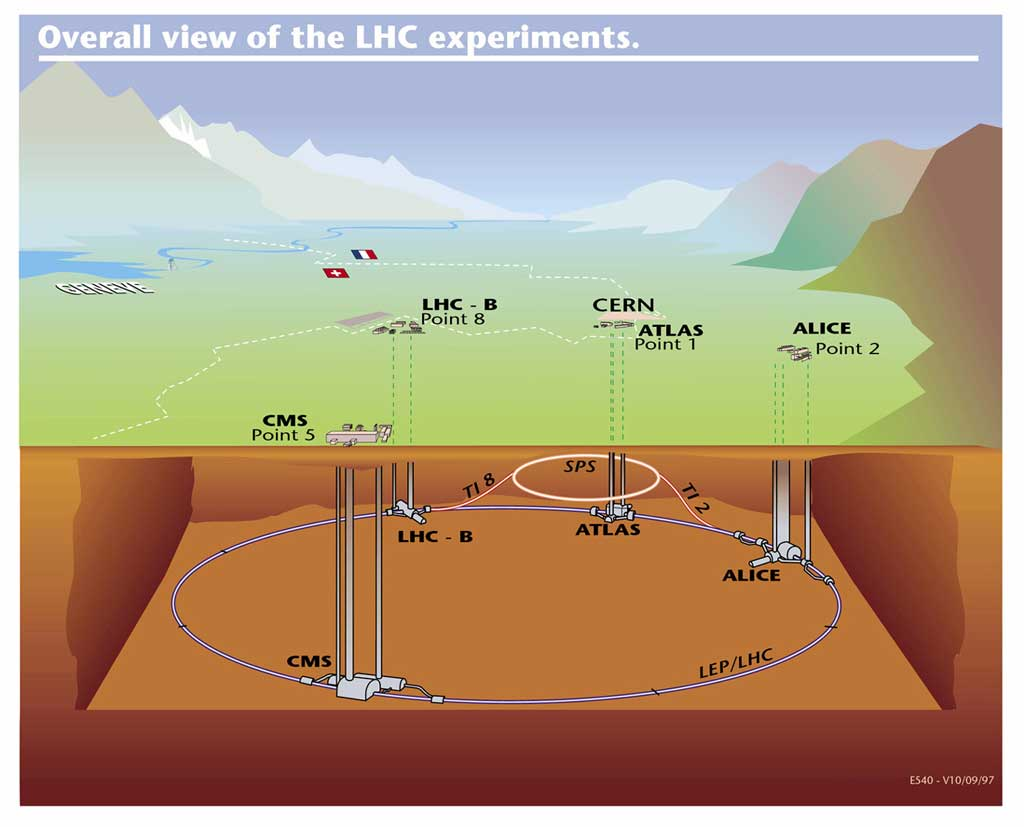
\includegraphics[width=10cm]{images/lhc-sim.png}
    \caption[Diagrama esquemático do túnel do LHC.]{Diagrama esquemático do
    túnel do LHC (Extraído de~\cite{ref:cern_www}).}
    \label{fig:lhc}
\end{figure}

O LHC começou a funcionar em 10 de setembro de 2008. Houve, porém, um acidente
que interrompeu sua operação. Um defeito na ligação elétrica entre dois
condutores causou um grande vazamento de hélio, que foi ventilado para dentro
do túnel, aumentando a temperatura em alguns dos equipamentos em torno de 100
graus Celsius~\cite{NATURE2008}. Apenas em 2009, as atividades foram
retomadas com a energia de centro de massa de $\sqrt{s} = 3,5~TeV$. Em
2010, colisões com a metade da energia projetada foram obtidas. A operação
ocorre de forma contínua até 2013, quando ocorrerá um grande período de
manutenção e a primeira fase de atualização dos
equipamentos~\cite{ref:ANDERSON2011}.

\subsection{Os experimentos do LHC}

Quatro grandes experimentos estão localizados ao redor da circunferência do LHC,
como foi mostrado na Figura~\ref{fig:lhc}: ATLAS~\cite{ATLAS2008, ref:BOELAERT2012},
CMS~\cite{ref:CMS}, LHCb~\cite{ref:SZUMLAK2010} e ALICE~\cite{ref:ALICE2008}. A
Figura~\ref{fig:experiments} ilustra os experimentos.


\begin{figure}[h!]
    \centering
    \begin{subfigure}[b]{0.45\textwidth}
        \centering
        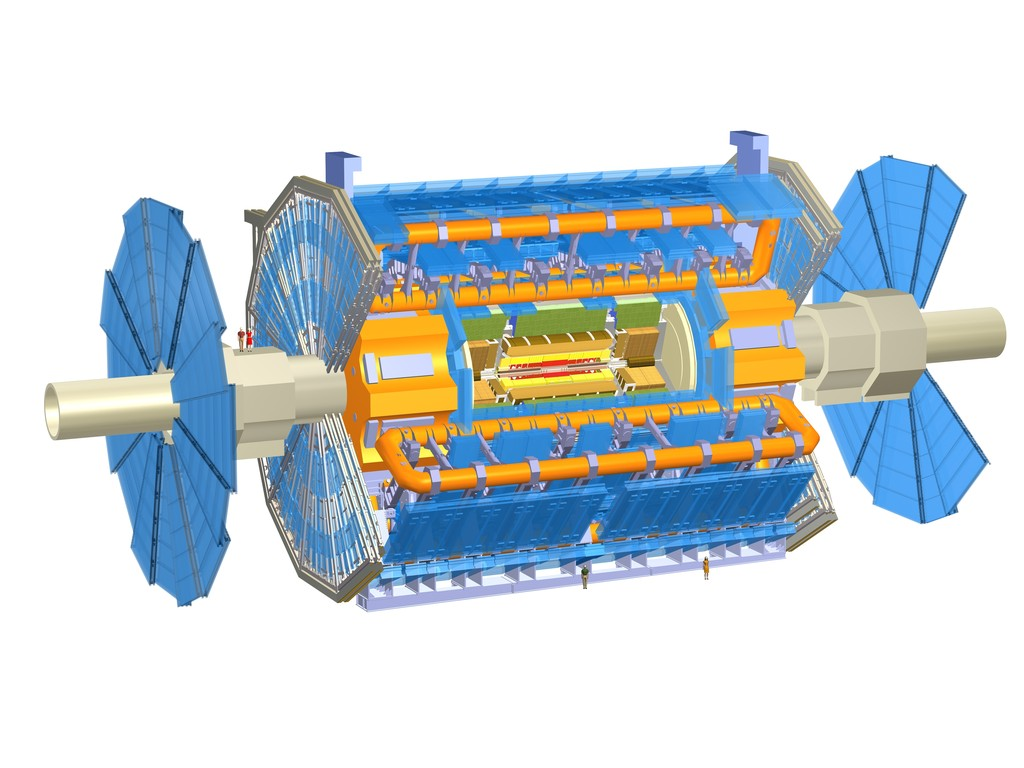
\includegraphics[width=\textwidth]{images/ATLAS.jpg}
        \caption{ATLAS}
    \end{subfigure}%
    ~
    \begin{subfigure}[b]{0.45\textwidth}
        \centering
        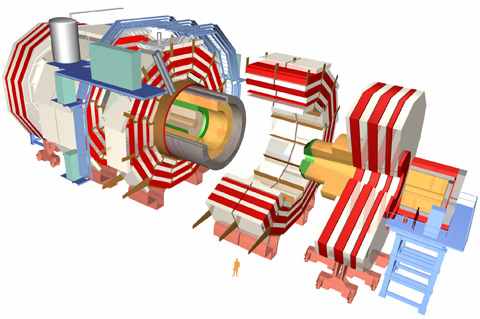
\includegraphics[width=\textwidth]{images/cms.jpg}
        \caption{ CMS}
    \end{subfigure}
    \\
    \begin{subfigure}[b]{0.45\textwidth}
        \centering
        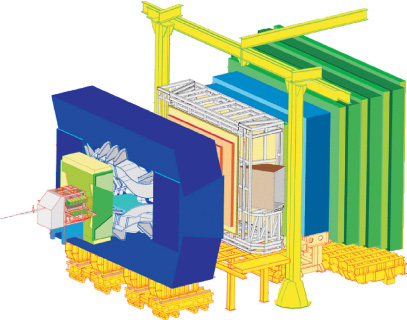
\includegraphics[width=\textwidth]{images/lhcb.jpg}
        \caption{LHCb}
    \end{subfigure}
    ~
    \begin{subfigure}[b]{0.45\textwidth}
        \centering
        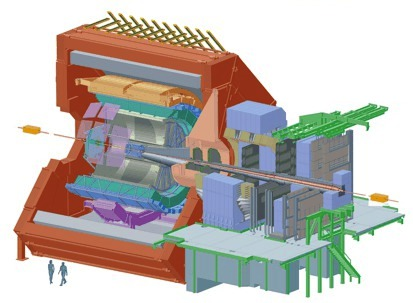
\includegraphics[width=\textwidth]{images/alice.jpg}
        \caption{ ALICE}
    \end{subfigure}
    \caption[Os quatro principais experimentos do LHCb]{Os quatro principais
    experimentos do LHCb (extraído de~\cite{ref:solans}).}
    \label{fig:experiments}
\end{figure}

O ATLAS e o CMS são experimentos de proposta geral, otimizados para estudar a
Nova Física com eventos na faixa dos TeV. Os outros dois foram projetados para
estudar fenômenos específicos: o LHCb realiza medições precisas do decaimento
do méson $B$ e o ALICE estuda colisões de íons de chumbo.


\section{O ATLAS}

O detector ATLAS tem aproximadamente 45~m de comprimento, mais de 25~m de altura
e pesa em torno de 7.000~T. É o resultado de uma colaboração de 3.000
pesquisadores de 38 países participantes representando 174 instituições
diferentes~\cite{ref:atlas_factsheet}\cite{GRAEL2011}.

Pode-se observar na Figura~\ref{fig:atlasschema} que este detector é composto
por sub-detectores distintos, cada um com características e
objetivos específicos.

\begin{figure}[H]
    \centering
    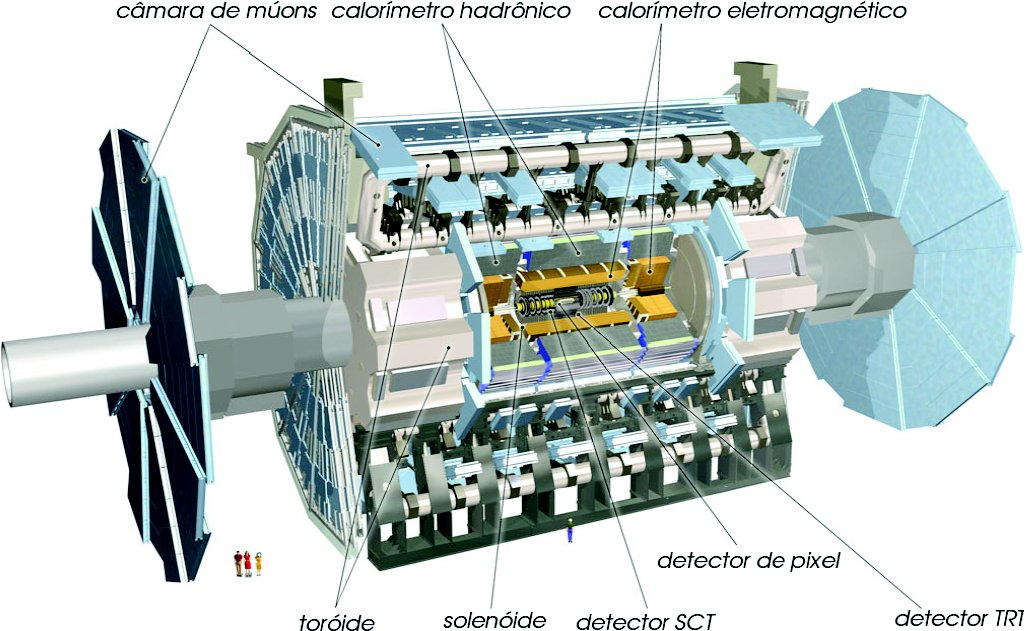
\includegraphics[width=0.8\textwidth]{images/ATLAS_esquema.png}
    \caption[Diagrama ilustrativo do detector ATLAS.]{Diagrama ilustrativo do
    detector ATLAS (adaptado de~\cite{ref:atlas_www}).}
    \label{fig:atlasschema}
\end{figure}

A Figura~\ref{fig:atlassection} apresenta um esquemático da seção transversal do
detector. Os números denotam os diferentes módulos. São eles:

\begin{figure}[H]
    \centering
    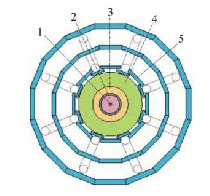
\includegraphics{images/atlas_transversal.png}
    \caption[Seção transversal do detector ATLAS.]{Seção transversal do detector
    ATLAS (extraído de~\cite{ref:TORRES}).}
    \label{fig:atlassection}
\end{figure}


\begin{enumerate}
    \item {\bf Tubo do Feixe:} localizado no centro do detector, aonde passam os
    feixes de prótons.
    \item {\bf Detector de Traços:} composto por uma infinidade de sensores
    altamente segmentados feitos de silício, determina com muita precisão a
    trajetória de partículas carregadas. Estas trajetórias são desviadas devido
    ao campo magnético presente no ATLAS. É possível dessa forma estimar o
    momento e a carga da partícula passante.
    \item {\bf Calorímetro Eletromagnético:} determina a energia e o perfil de
    deposição de energia de partículas eletromagnéticas, como, por exemplo,
    elétrons e fótons. Está dividido em quatro camadas, cada uma com
    granularidade distinta.
    \item {\bf Calorímetro Hadrônico:} determina a energia e o perfil de
    deposição de energia de partículas hadrônicas, como por exemplo os prótons.
    Está dividido em 3 camadas  com granularidades distintas.
    \item {\bf Espectrômetro de múons:} Os múons são cerca de 200 vezes mais
    pesados do que elétrons. Por essa razão, estas partículas depositam pouca
    energia ao cruzar o campo elétrico de átomos que estejam no seu caminho.
    Não sendo absorvidas pelos detectores.  O Espectrômetro é composto pela
    câmaras de múon~\cite{ref:atlas2009}, onde um campo magnético é utilizado
    para curvar a trajetória dos múons. Este procedimento aliado a um poderoso
    sistema de detecção de traço específico, permite a medição do momento da
    partícula.

\end{enumerate}

O Calorímetro Hadrônico e o Espectrômetro de múons serão descritos
detalhadamente ao longo desse capítulo.

\subsection[Sistema de Coordenadas]{Sistema de Coordenadas do ATLAS}

O sistema de coordenadas do ATLAS é um sistema cartesiano que segue a regra da
mão direita. Nesse sistema, apresentado na Figura~\ref{fig:coordinates},
encontram-se~\cite{EGEDE1998}:


\begin{itemize}
    \item o eixo $x$, com lado positivo apontado para o centro da
    circunferência do anel do LHC,
    \item o eixo $z$, seguindo a direção do feixe de partículas,
    \item o eixo $y$, apontando para cima.
\end{itemize}

\begin{figure}[htpb!]
    \centering
    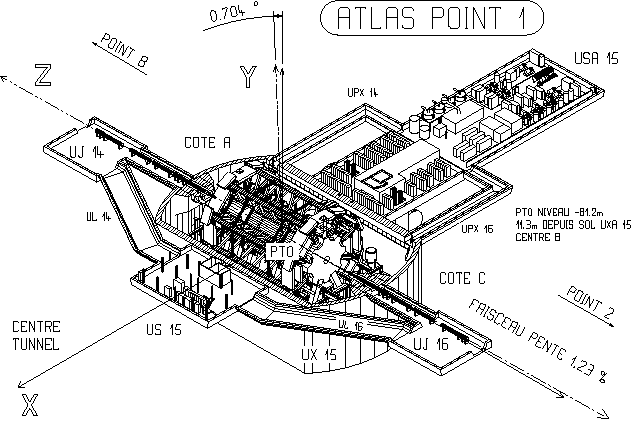
\includegraphics[width=\textwidth]{images/atlas_coordinate_system.png}
    \caption[Sistema de coordenadas do ATLAS]{Sistema de coordenadas do ATLAS (extraído
    de~\cite{EGEDE1998}).}
    \label{fig:coordinates}
\end{figure}

Ao analisar colisões, o sistema cartesiano, mostra-se ineficiente. Nestes
casos, é comum utilizar um sistema que acompanha a direção das partículas
provenientes do ponto de colisão. Assim, são definidas três novas coordenadas
a partir de transformações não-lineares de $x$, $y$ e $z$:

\begin{equation}
    \phi = \arctan\left(\frac{x}{y}\right)
\end{equation}
\begin{equation}
    \Theta = \arctan\left(\frac{x}{z}\right)
\end{equation}
\begin{equation}
    \eta = -\log \left(\tan\left(\frac{\Theta}{2}\right)\right)
\end{equation}

São adicionadas às coordenadas originais o ângulo azimutal $\phi$ (ao
redor de $z$) e a pseudo-rapidez ($\eta$), que representa a direção da projeção
da partícula, após a colisão.

\subsection{Calorímetro Hadrônico de Telhas}

Calorímetros são fundamentais em detectores hadrônicos de propósitos
gerais~\cite{WIGMANS2000}.  O Calorímetro Hadrônico de
Telhas~\cite{ARIZTIZABAL1994}, conhecido como \emph{TileCal}, desempenha esse
papel.

O sistema de calorimetria do ATLAS é capaz de estimar com grande precisão
medidas de energia e posicionamento de elétrons, prótons, hádrons, taus e jatos.
Também colaboram na identificação e reconstrução de
múons~\cite{AAD2010READINESS}. O TileCal foca na obtenção de medidas precisas de
hádrons, jatos, taus e energia transversa faltante~\cite{MERMOD2008}.

Este calorímetro utiliza cintiladores plásticos como material ativo e ferro
como material que absorve. Compreende a região de pseudo-rapidez $-1,7 < \eta <
1,7$, sendo subdividido em três regiões: uma central  ($-1,0 < \eta < 1,0$),
chamada barril longo~(LB) e dois barris estendidos (EB) localizados nos flancos
do detector ( $0,8 < \|\eta\| < 1,7$), como pode ser visto na
Figura~\ref{fig:tilecalschema}. Ambos, barril longo e estendido, são
segmentados em 64 fatias (módulos) em $\phi$ correspondendo a uma granularidade
$\Delta\phi$ de aproximadamente $0,1$~radianos~\cite{DETECTOR1996TECHNICAL}.

\begin{figure}[htpb!]
    \centering
    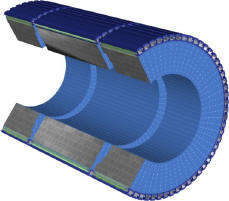
\includegraphics{images/TILECAL_modules_schema.jpg}
    \caption[Diagrama esquemático do TileCal]{Diagrama esquemático do TileCal (extraído
    de~\cite{ref:atlas_www}).}
    \label{fig:tilecalschema}
\end{figure}

Cada módulo é segmentado em três camadas radialmente. Há também a variação
$\Delta\eta$,  igual a $0,1$ nas duas primeiras camadas (denominadas A e BC) e
$0,2$ na terceira camada (denominada D). Deste modo, $\phi$, $\eta$ e a
segmentação radial definem as três dimensões das células do TileCal.  A Figura
~\ref{fig:tilecalgeometry} mostra a distribuição das células dentro de um
módulo.

\begin{figure}[htpb!]
    \centering
    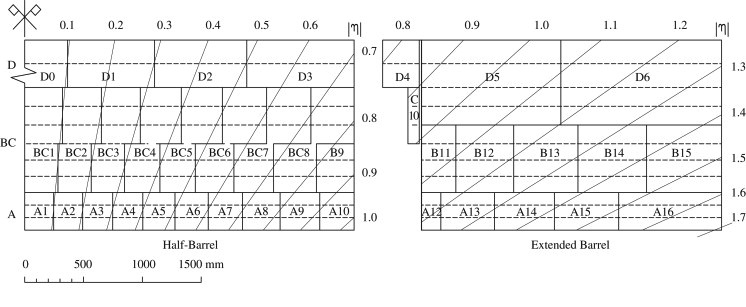
\includegraphics[width=\textwidth]{images/tile_geometry.jpg}
    \caption[Geometria de células do TileCal]{Geometria de células do TileCal.}
    \label{fig:tilecalgeometry}
\end{figure}


Cada célula possui dezenas de placas de ferro e telhas cintilantes. Fibras
óticas deslocadoras de comprimento de onda  (fibras WLS) acopladas às telhas nas
bordas azimutais das células, mostradas na Figura~\ref{fig:tilecalslice},
coletam a luz produzida e a levam até dois tubos fotomultiplicadores
diferentes (PMTs). Cada tubo está conectado a um canal de aquisição, garantindo a
redundância necessária.


A arquitetura de aquisição do TileCal divide o detector em quatro partições. O
barril longo é dividido em duas partições (LBA e LBC) no local entre  plano
perpendicular ao tubo do feixe e o ponto de colisão, e cada barril estendido é
uma partição separada (EBA e EBC)~\cite{AAD2010READINESS}.

A eletrônica de aquisição está localizada em ``gavetas'' inseridas na parte
externa do perímetro do calorímetro. Cada gaveta possui normalmente 45
canais de leitura no barril longo e 32 no barril estendido.

\begin{figure}[htpb!]
    \centering
    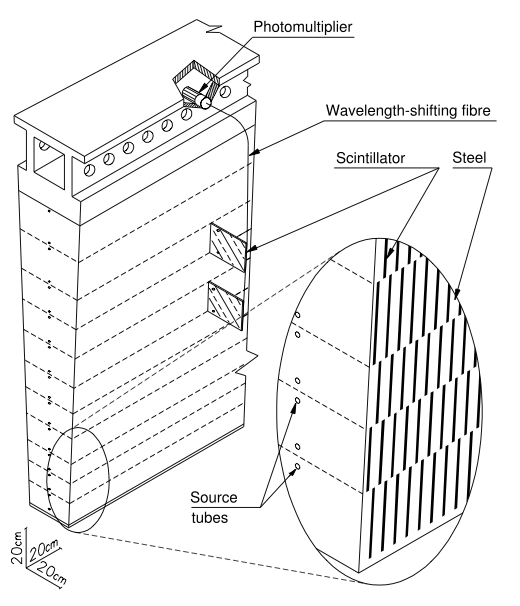
\includegraphics[width=0.5\textwidth]{images/tile_slice.jpg}
    \caption[Estrutura de absorção e amostragem do TileCal]{Estrutura de
    absorção e amostragem do TileCal~(extraído de~\cite{ATLAS2008}).}

    \label{fig:tilecalslice}
\end{figure}

A Tabela~\ref{table:tilefacts} resume a quantidade de canais, de células e de
saídas de trigger para cada tipo de barril.


\begin{table}[htbp!]
  \centering
  \begin{tabular}{ l  r  r  r  }
      \toprule
                         & Canais & Células & saídas de \emph{Trigger}\\
      \midrule
        Barril Longo     & 5760 & 2880 & 1152 \\
        Barril estendido & 4076 & 2302 &  928 \\ [2ex]
        {\bfseries Total}            & 9836 & 5182 & 2080 \\
      \bottomrule
  \end{tabular}
  \caption{Número de canais, células e saídas de Trigger do TileCal.}
  \label{table:tilefacts}
\end{table}

Tanto a eletrônica de \emph{front-end} como as fontes de baixas tensões (LVPS, do
inglês \emph{Low Voltage Power Supplies}) estão localizadas dentro das gavetas e,
portanto, foram projetadas para operar sob condições de elevada radiação e forte
campo magnético~\cite{hruska2007radiation,ARABIDZE2011}.

Os sinais luminosos adquiridos são transformados em  pulsos elétricos
através de um circuito passivo (\emph{shaper})~\cite{AMES1998}. O pulso é
condicionado para ter uma largura constante, de 50~ns, e amplitude proporcional
à intensidade da quantidade de luz absorvida~\cite{ANDERSON2005}. O pulso
formado é disponibilizado tanto amplificado com um  ganho elevado (HG, do
inglês \emph{high gain}), como também, inalterado (LG, do inglês \emph{low
gain}). A razão nominal entre os dois ganhos é aproximadamente
64:1~\cite{AAD2010READINESS}. O \emph{shaper}, o circuito de amplificação e o
sistema de injeção de cargas para calibração (CIS) estão localizados em um
pequeno circuito impresso conhecido como \emph{3in1 card}~\cite{ANDERSON2005}.

Os sinais HG e LG são amostrados na frequência de 40~MHz utilizando um conversor
analógico digital de 10 bits de faixa dinâmica presente em uma unidade de
gerenciamento de dados~(DMU, \emph{Tile data management unit}). Essa unidade
contêm um \emph{pipeline} de memória que armazena o sinal amostrado por até
6,4~$\mu$s. 

Posteriormente, as amostras são enviadas via cabos de fibra ótica para a
eletrônica de \emph{backend}, localizada fora da caverna principal do
experimento ATLAS. A eletrônica de \emph{backend} determina o período e a
energia do canal das amostras digitalizadas.

A placa \emph{3in1} ainda possui um circuito integrador projetado para medir a
corrente numa determinada PMT durante sessões de calibração com Césio
137~\cite{ANDERSON2009} e interações próton-próton em eventos de \emph{minimum
bias} ocorridos no LHC~\cite{AAD2010READINESS}. O período de integração é de
aproximadamente $14~ms$ e um conversor de 12 bits é utilizado para leitura. A
Figura~\ref{fig:3in1} apresenta o esquemático da placa \emph{3in1} onde todos
seus subsistemas podem ser observados.

\begin{figure}[htpb!]
    \centering
    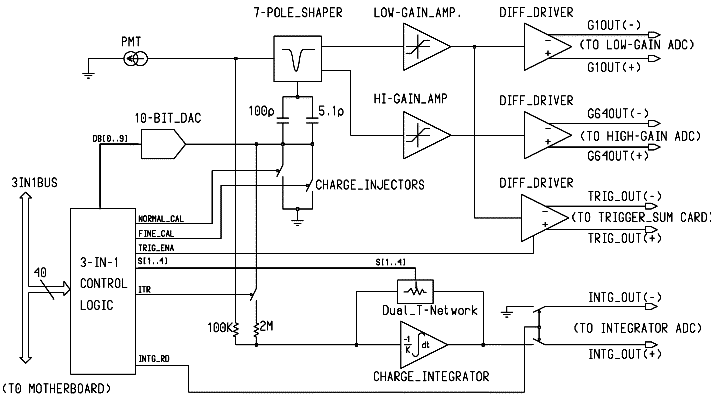
\includegraphics[width=\textwidth]{images/3in1.png}
    \caption[Diagrama de blocos da placa \emph{3in1}]{Diagrama de blocos da
    placa \emph{3in1}(extraído
    de~\cite{ANDERSON2005}).}
    \label{fig:3in1}
\end{figure}

Existem circuitos somadores distribuídos ao longo de uma gaveta e estes são
responsáveis pela interface entre o TileCal e o primeiro nível do sistema de
filtragem do ATLAS~\cite{CERQUEIRA2007}. Cada somador recebe os sinais
analógicos disponibilizados por até 6 placas \emph{3in1}, o que  corresponde a
células localizadas no mesmo intervalo de $\eta$. O sinal de \emph{trigger},
que corresponde a uma ``torre'' de células com  $\Delta\eta \times \Delta\phi =
0,1 \times 0,1$, é formado pela soma analógica dos sinais de entrada. Ele é
posteriormente transmitido junto com  sinais provenientes dos demais
calorímetros do ATLAS para a área externa da caverna do experimento, através de
longos cabos.

Além do sinal da torre, o circuito somador também fornece uma leitura
amplificada da leitura de LG das PMTs localizadas nas células da camada D. Esta
saída é conhecida como ``sinal de múon''. Este sinal é amplificado com um
ganho igual a 255 em relação ao sinal de LG. É um sinal unipolar diferencial,
com excursão máxima de 4Vpp~\cite{CERQUEIRA2007}.

Vale notar que as células da camada D possuem baixa atividade
hadrônica~\cite{CIODARO2009} e, por isso, entende-se que as informações
adquiridas nela  possam ser utilizadas para mitigar o ruído de fundo na
aquisição de múons. Foi esta possibilidade que motivou o presente trabalho de
pesquisa.



\subsection{Sistema de Múons}

O Espectrômetro de Múon ~(MS) compõe a parte externa do ATLAS. Foi projetado
para detectar partículas carregadas que passem pela seção dos calorímetros e
para medir o momento delas na pseudo-rapidez $\|\eta\| < 2,7$~\cite{ATLAS2008}.
Seus principais objetivos para operação são ~\cite{Aad:1275998}:

\begin{itemize}
    \item prover uma medida independente do momento de múons com uma incerteza
    estimada no momento transverso ($p_T$) variando de 3\% em 100~GeV até cerca
    de 10\% em 1~TeV; 
    \item detectar múons com momentos transversos desde maiores que 3~GeV
    devido a perda de energia nos calorímetros~\cite{ATLAS2008}.
\end{itemize}

O momento de um  múon é determinado a partir da medição de sua trajetória
curvilínea ao passar pelo campo magnético toroidal. Esta trajetória é sempre
perpendicular em relação a principal componente do campo magnético,  o que faz
o cálculo do momento transverso ser independente de $\eta$. O campo magnético é
gerado por três toroides, um na região do barril ($\|\eta\| < 1,1$) e dois nas
regiões dos ``\emph{end-caps}'' ($1,1 < \|\eta\| < 2,7$) com campo total entre 2
e 8~Tm~\cite{Aad:1275998}.

A curvatura do múon é calculada por meio de três estações com câmaras
localizadas ao longo de sua trajetória. Cada estação possui uma acurácia de
$50~\mu$m~\cite{MUONTDR1997}. A Figura~\ref{fig:muonspec} apresenta uma
visualização esquemática do espectrômetro.



\begin{figure}[htpb!]
    \centering
    \begin{subfigure}[b]{\textwidth}
        \centering
        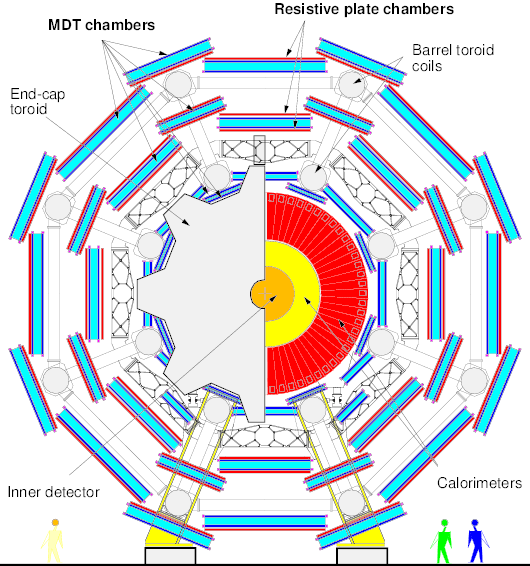
\includegraphics[width=0.9\textwidth]{images/ATLAS-muon-xy-tdr.png}
        \caption{Projeção x-y.}
        \label{fig:muonspecxy}
    \end{subfigure}
    \begin{subfigure}[b]{\textwidth}
        \centering
        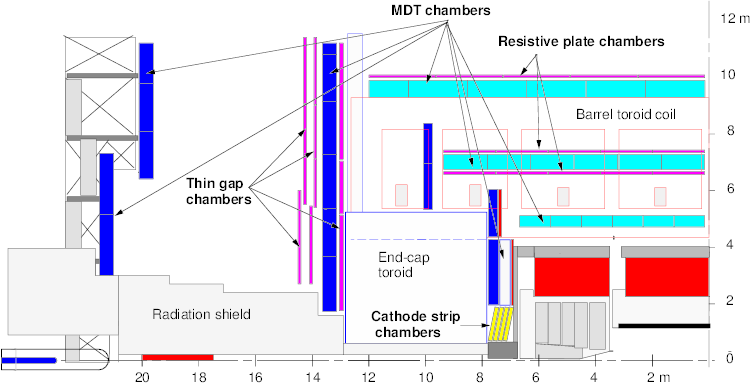
\includegraphics[width=0.9\textwidth]{images/ATLAS-muon-rz-tdr.png}
        \caption{Projeção y-z.}
        \label{fig:muonspecyz}
    \end{subfigure}~\\%
    \caption[Visualização gráfica do Espectrômetro de múons.]{Esquemático do
    espectrômetro de múon (Extraído de~\cite{MUONTDR1997}}).
    \label{fig:muonspec}
\end{figure}

As câmaras são divididas em quatro tecnologias: \emph{Cathode Strip Chambers}
(CSC), \emph{Monitored Drift Tubes} (MDT), \emph{Resistive Plate Chambers}
(RPC) e \emph{Thin Gap Chambers} (TGC). O RPC e o TGC são utilizados como
detectores de múons no primeiro nível de filtragem do ATLAS. Já o MDT e CSC são
utilizados para uma medida com alta resolução, porém suas informações só são
utilizadas em eventos pré-selecionados. Como o MDT e o RPC encontram-se na
parte do barril, são de maior interesse para esse trabalho.


\subsubsection*{\emph{Monitored Drift Tubes} (MDT)}

As câmaras  MDT são responsáveis no barril pelas medições das trajetórias
curvilíneas de múons. Elas ocupam uma área de $5.500~\text{m}^2$ na região de
rapidez $\|\eta\|<2,7$.

O elemento básico de detecção é um tubo cilíndrico de alumínio com 30~mm de
diâmetro. Em seu interior há um fio de tungstênio-rênio com 50~$\mu$m de
diâmetro, concêntrico com uma acurácia de $10~\mu$m, mantido a 3.080~V. O tubo é
preenchido com um gás não-inflamável composto por argônio~(93\%) e gás
carbônico~(7\%)~\cite{RIEGLER2000}. Os elétrons ionizados pela passagem de uma
partícula carregada são coletados pelo fio condutor, gerando pulsos de corrente
elétrica. Os elétrons que chegam mais rápido ao centro do tubo são exatamente os
que se localizam, no início do processo, no ponto onde a distância entre a
trajetória da partícula e do fio é mínima. Uma série de outros elétrons se
aproximam do fio, gerando picos de corrente por um determinado tempo. Contudo,
apenas o primeiro pico é considerado. A Figura~\ref{fig:mdttube} explica esse
processo. As linhas pontilhadas exemplificam o caminho percorrido por diversos
elétrons, enquanto a linha contínua indica a passagem de um múon.  O gráfico
ilustra que o primeiro pico corresponde ao ponto mais próximo em que partícula
passou em relação ao centro do tubo. Como pode-se supor, a eletrônica de
aquisição e o sistema de alimentação encontram-se nas extremidades do fio, em
oposição entre si~\cite{ATLAS2008}.


\begin{figure}[htpb!]
    \centering
        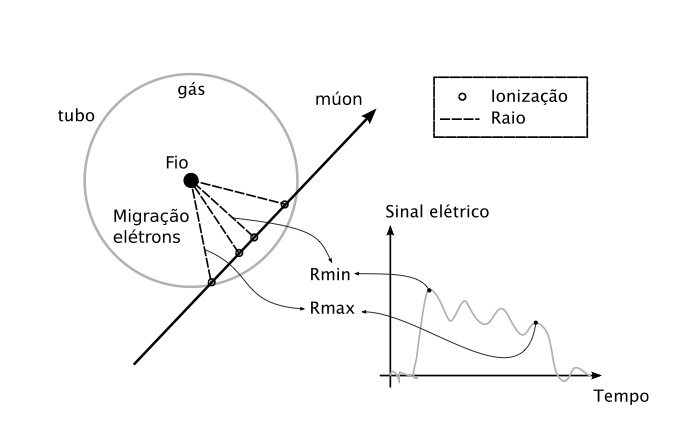
\includegraphics{images/mdt_ion.png}
        \caption[Funcionamento de um tubo do MDT para estimar de maneira precisa a
        trajetória de um múon.]{ Funcionamento de um tubo
        do MDT para estimar de maneira precisa a trajetória de um múon~(adaptado
        de~\cite{MUONTDR1997}).}
        \label{fig:mdttube}
\end{figure}



As câmaras de MDT são montadas a partir de seis camadas de tubos dispostos em um
chassi, três camadas de cada lado, como pode ser visto na
Figura~\ref{fig:mdtchamber}. Os tubos são alinhados de tal maneira que a
espessura do material \emph{multilayer} é em torno de 88~mm. Deste modo, cada
câmara registra seis coordenadas para a trajetória de cada partícula. Na
Figura~\ref{fig:muonspecxy} é possível observar o posicionamento das câmaras em
torno do eixo z.

\begin{figure}[htpb!]
    \centering
        \includegraphics[width=0.8\textwidth]{images/MDTChamber.png}
        \caption[Esquemático de uma câmara MDT.]{Esquemático de uma câmara
        MDT~(retirado de~\cite{MUONTDR1997}).}
        \label{fig:mdtchamber}
\end{figure}


\subsubsection*{\emph{Resistive Plate Chambers} (RPC)}

As câmaras de MDT são relativamente lentas para serem usadas pelo primeiro
nível de filtragem do ATLAS. Por isso, na parte central do barril também
encontram-se as câmaras RPC. Elas estimam o $p_T$ com baixa resolução, porém
com rápida resposta, o que preenche os requisitos do sistema de
filtragem~\cite{MUONTDR1997}. A Figura~\ref{fig:rpclocation} mostra uma seção
do detector e a localização dos RPC (coloridos) em relação aos MDTs. A
Tabela~\ref{table:rpc_segmentation} apresenta a segmentação do sistema RPC
através da contagem de câmaras e da distância radial de cada RPC.

\begin{figure}[htpb!]
    \centering
        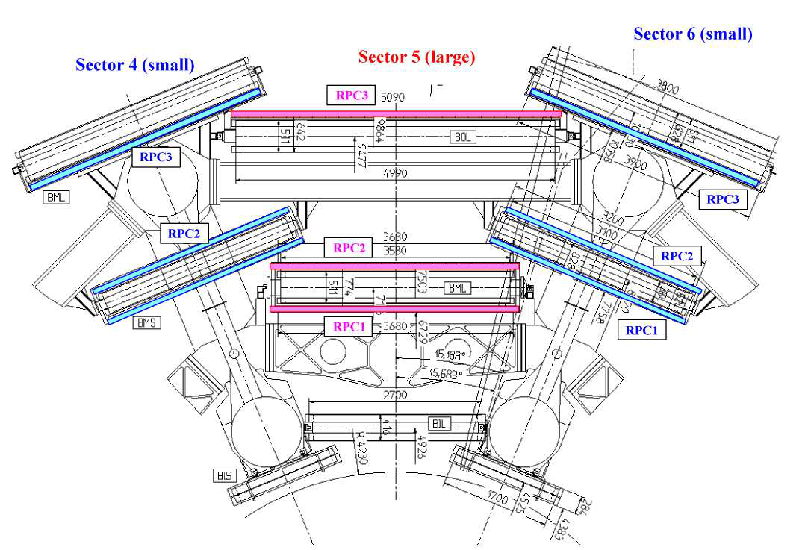
\includegraphics[width=\textwidth]{images/rpc_location.png}
        \caption[Localização dos RPCs na Seção transversal da parte superior do
        barril longo.]{Seção transversal da parte superior do barril longo com
        os RPCs destacados. Na camada do meio encontram-se os RPC1 e RPC2 (ou
        \emph{pivot}), localizados acima e abaixo de um MDT específico. Já o RPC3
        localiza-se acima de um MDT na seção grande e abaixo na outra~(retirado
        de~\cite{Aad:1275998}). As dimensões estão em mm.}
        \label{fig:rpclocation}
\end{figure}


Cada plano do RPC é um conjunto de duas chapas resistivas feitas de baquelite
(resina plástica resistente ao calor). Essas chapas são postas distanciadas uma
da outra por 2~mm. O espaço é preenchido por um gás ionizado. O campo
elétrico aplicado entre as duas placas é igual $ 4,9~kV/mm$~\cite{ATLAS2008}.
Fitas metálicas são dispostas ao longo de $\eta$ e $\phi$, fornecendo a
granularidade requerida pelo ATLAS~\cite{MUONTDR1997, POLINI2012}.

As partículas que cruzam o detetor ionizam o gás do RPC. Elétrons são liberados
e atraídos pelo campo elétrico até as extremidades da câmara, onde são coletados
pelas fitas metálicas. Os sinais das fitas são adquiridos por uma eletrônica
simples que compara com padrões previamente determinados~\cite{MUONTDR1997}. A
distribuição espacial e temporal dos pontos sensibilizados pela passagem de um
múon é suficiente para estimar o seu momento transverso~\cite{ANULLI2009}.

\begin{table}[htbp!]\footnotesize
  \centering
  \tabcolsep=0.08cm
  \begin{tabular}{ m{1.5cm}   m{1.5cm}  m{1.5cm}  m{1.5cm}  m{1.5cm} m{1.5cm} m{1.5cm}  m{1.5cm}  m{1.5cm}  }
       \multicolumn{1}{c}{}& \multicolumn{4}{c}{Setor pequeno}& \multicolumn{4}{c}{Setor Grande} \\
        \cmidrule(r){2-5}
        \cmidrule(r){6-9}
      Nome & Unidades & Câmaras & Raio & Distância ao Pivot & Unidades & Câmaras & Raio & Distância ao Pivot \\
      \midrule
      RPC1 & 148 & 84 & 7820  & 545  & 149 & 94 & 6800 & 678 \\
      RPC2 & 148 & 84 & 8365  &      & 149 & 94 & 7478 &     \\
      RPC3 & 176 & 92 & 10229 & 1864 & 192 & 96 & 9832 & 2354\\
      \bottomrule
  \end{tabular}
  \caption{Segmentação do sistema RPC com 544 câmaras e 962 unidades. Todas as
  dimensões estão em mm.}
  \label{table:rpc_segmentation}

\end{table}


\subsubsection*{Geometria do RPC}

As três camadas do MS estão distribuídas de acordo com a distância do feixe de
partículas do ATLAS. A Figura~\ref{fig:muonsector} mostra a divisão lógica e a
numeração dada ao MS. Essas camadas são chamadas de \emph{inner}, \emph{middle}
e \emph{outer} localizadas respectivamente a 3,5~m, 5~m e 7~m. O espectrômetro
é dividido azimutalmente em 64 setores (chamados setores de \emph{trigger}),
pequenos ou grandes.

\begin{figure}[htpb!]
    \centering
    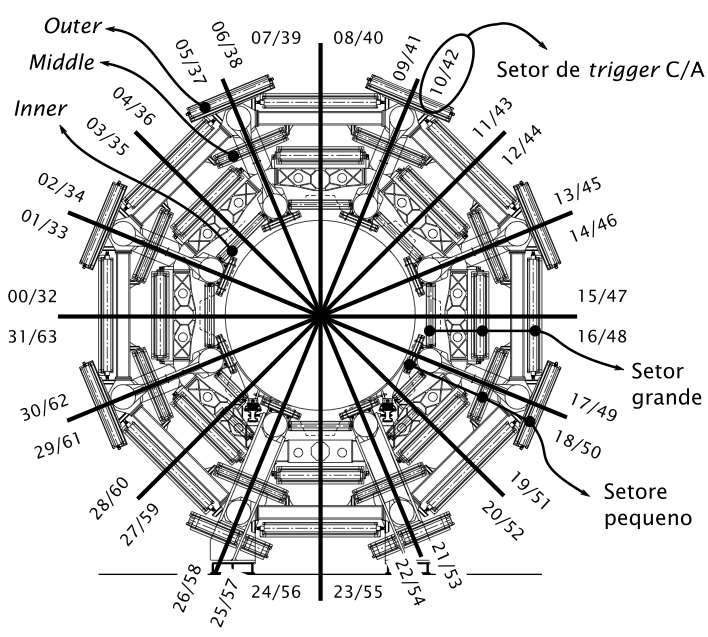
\includegraphics[width=0.8\textwidth]{images/muon_sectors.png}
    \caption{Setores de \emph{trigger} do Espectrômetro de Múons}
        \label{fig:muonsector}
\end{figure}

Cada câmara no plano \emph{pivot} define duas regiões de \emph{trigger} em
$\eta \times \phi$, chamadas PAD~\cite{ANULLI2009}, com granularidade $0,2
\times 0,2$.  Dentro de uma PAD são definidas regiões de interesse (RoI, do
inglês \emph{Regions of Interest}) que ocupam aproximadamente $0,1 \times 0,1$
em $\eta \times \phi$. A Figura~\ref{fig:muonroi} mostra o mapeamento dos RPC
em RoIs. Existem áreas em $\phi$ onde diferentes setores se sobrepõem. Múons
que cruzam essas regiões são registrados por ambas, porém somente uma será
considerada pela eletrônica de aquisição, acabando com a
ambiguidade~\cite{ANULLI2009}.


\begin{figure}[htpb!]
    \centering
    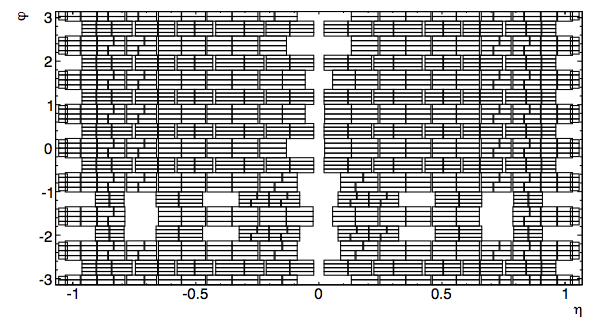
\includegraphics[width=0.8\textwidth]{images/muonroi.png}
    \caption{Mapa de RoIs para o RPC}
        \label{fig:muonroi}
\end{figure}

%%End of chapter
%%%%%%%%%%%%%%%%%%%%%%%%%%%%%%%%%%%%%%%%%%%%%%%%%%%%%%%%%%%%%%%%%%%%%%%%%%

%\subsection{A descoberta do bóson de Higgs}
%\begin{figure}[htpb!]
%    \centering
%    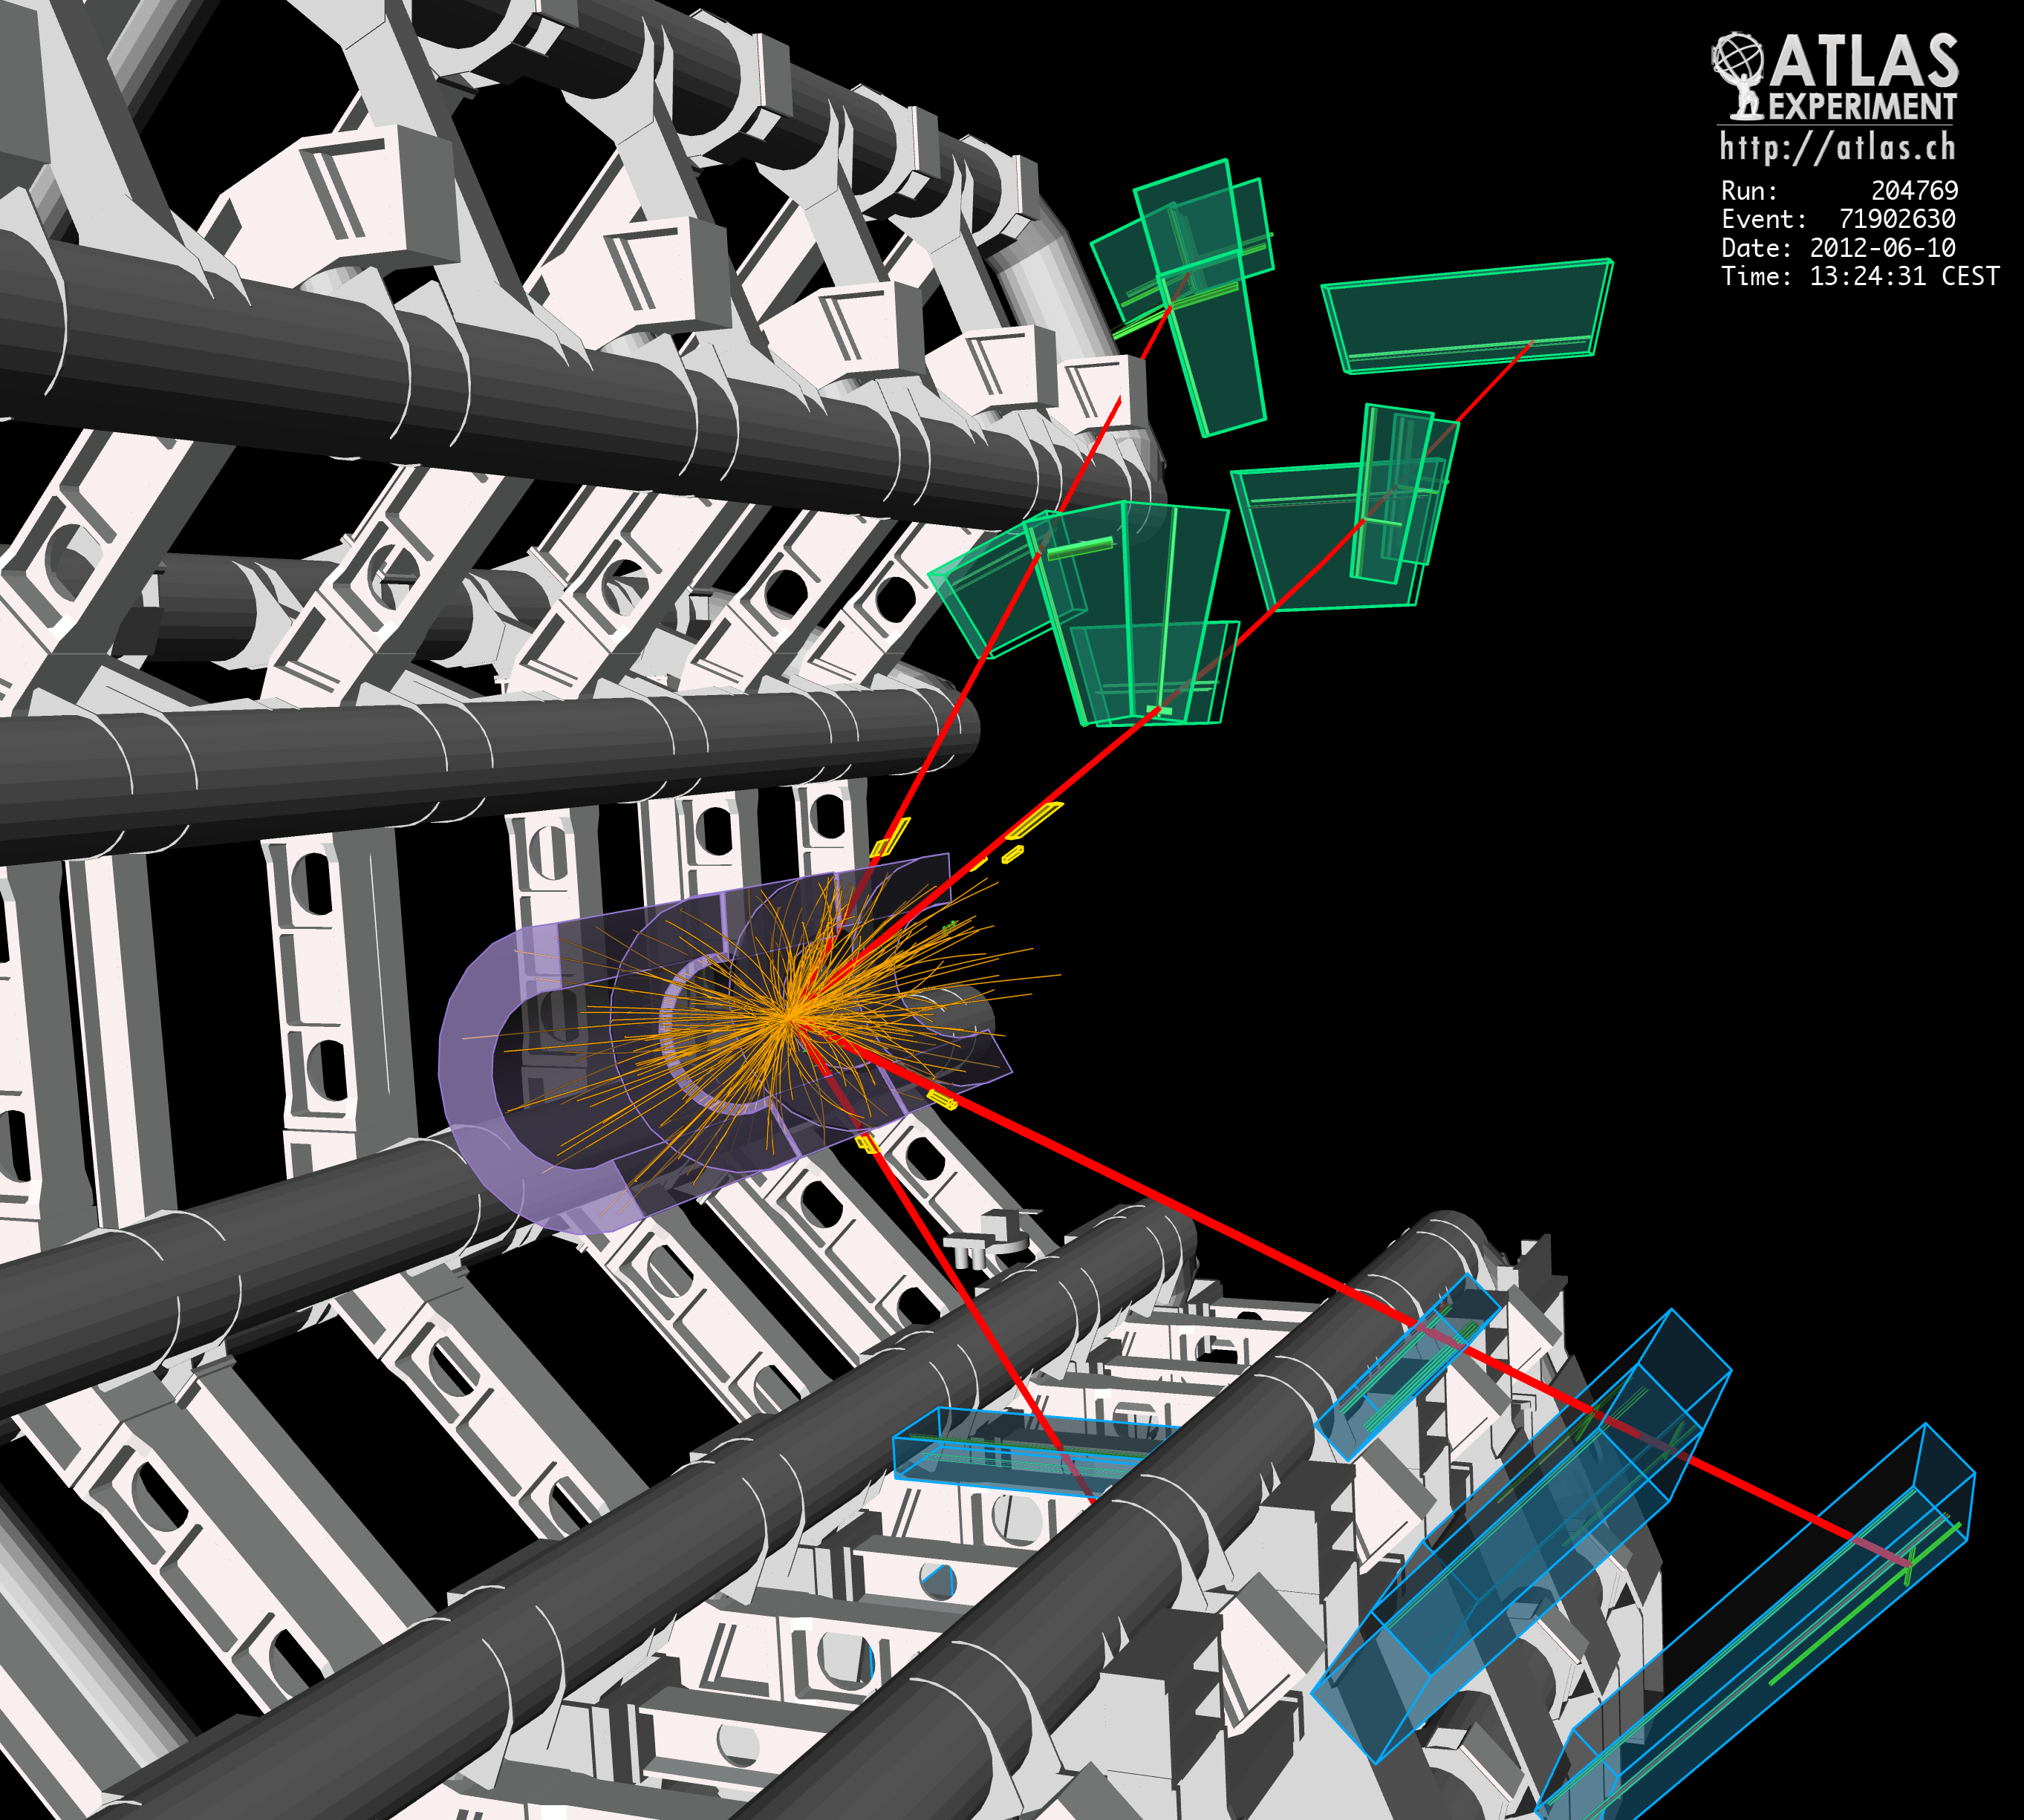
\includegraphics[width=\textwidth]{images/run204769_evt71902630_MSonly_hres.png}
%    \caption{Reprodução de um evento candidato a $H \rightarrow 4\mu$ (extraído
%    de~\cite{ref:atlas_www}).}
%\end{figure}
